\chapter{Hamiltonovská kružnice}\label{Hamiltonovská kružnice}

Jednou z možností, jak docílit úspěšného dokončení hry Snake, je donutit hada v každé iteraci projít každé políčko právě jednou (viz Obrázek \ref{fig:Hamiltonian_cycle_example}). Takovým způsobem zamezíme tomu, že had narazí sám do sebe, a zároveň, že si had při prodlužování nezamezí úplně přístup k nějaké části hracího pole, tedy že i po maximálním prodloužení zůstane každé políčko dosažitelné. Takové cestě se v grafové teorii říká Hamiltonovská kružnice~\cite{HamiltonianCycleGFG}. Nalezení Hamiltonovské kružnice je ovšem výpočetně náročný problém (jinak známý jako problém obchodního cestujícího), konkrétně patří do třídy \(NP\)- úplných problémů. To znamená, že časová složitost nalezení Hamiltonovské kružnice je \(O(n!)\) a složitost ověření správnosti řešení je také \(O(n!)\).

\begin{figure}[!ht]
    \centering
    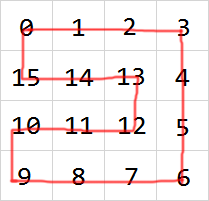
\includegraphics[width = 5cm]{Images/Hamiltonian_cycle_examle.png}
    \caption[Dostupné z: \url{https://gamedev.stackexchange.com/questions/133460/how-to-find-a-safe-path-for-an-ai-snake}]{Příklad hamiltonovské kružnice pro hrací pole \(4 \times 4\)}
    \label{fig:Hamiltonian_cycle_example}
\end{figure}

\section{Třídy složitostí}
Jedním z nejslavnějších a nejtěžších problémů, který v informatice existuje, je problém \(P\) versus \(NP\). \(P\) označuje množinu všech algoritmických problémů, které je možné vyřešit deterministickým Turingovým strojem v polynomiálním čase. Polynomem~\cite{MathTutorFunctions2025} rozumíme matematický výraz ve tvaru:
\[
P(x) = a_n x^n + a_{n-1} x^{n-1} + \cdots + a_1 x + a_0
\]
kde \(a_0, a_1, \dots, a_{n-1}, a_n\) jsou reálné koeficienty a \(n\) je nezáporné celé číslo, které určuje stupeň polynomu. Příkladem polynomu může být: \(4x^3 + 5x^2 - 8\). 

Vyřešit problém v polynomiálním čase znamená, že doba, kterou algoritmus potřebuje k vyřešení problému, je omezena polynomem závislém na velikosti vstupu. Protože Landau-\\ova~notace~\cite{BigONotationGFG} (známá také jako notace velké \(O\)) zanedbává konstantní koeficienty a zaměřu-\\je se pouze na nejvyšší prvek polynomu, můžeme říci, že algoritmus řešící problém v polynomiálním čase má časovou složitost \(O(n^k)\), kde \(n\) je velikost vstupu a \(k\) je konstanta označující stupeň polynomu. To znamená, že doba běhu algoritmu roste nejvýše polynomi-\\álně vzhledem k velikosti vstupu. To znamená, že pro dostatečně velké \(n\) je růstová rychlost takové funkce pomalejší než exponenciální \(O(2^n)\) nebo faktoriálové \(O(n!)\) složitosti, což činí problémy z třídy \(P\) prakticky řešitelnými. Pro problémy z třídy \(P\) vždy existuje řešení, které problém řeší v polynomiálním čase, a existuje i způsob, jak v polynomiálním čase ověřit správnost výsledku. 

Problémy třídy \(NP\) definujeme jako ty, které jsou v polynomiálním čase řešitelné nedeter-\\ministickým Turingovým strojem, jehož myšlenka je pouze hypotetická. Zjednodušeně můžeme říci, že \(NP\) problémy jsou takové, jejichž správnost řešení dokážeme ověřit v polynomiálním čase, ale nedokážeme přesně určit, zdali lze řešení v polynomiálním čase najít.

Všechny problémy v \(NP\) dokážeme redukovat na jiné problémy ve třídě \(NP\), to znamená, že pokud bychom dokázali najít řešení v polynomiálním čase pro jeden problém z \(NP\), dokázali bychom tím, že všechny problémy v \(NP\) lze řešit v polynomiálním čase. To by ale také znamenalo, že \(P = NP\). Většina odborníků se ovšem domnívá, že takový efektivní algoritmus neexistuje, a proto je většina přesvědčena o tom, že rovnost neplatí, tedy že  $P \neq NP$.

Třídy složitosti můžeme dále dělit na \(NP\)- úplné a na \(NP\)- těžké problémy~\cite{demaine2016complexity}. \(NP\)- těžké problémy popisují třídu, ve které jsou problémy těžké alespoň jako všechny \(NP\) složité problémy. To znamená, že bude obsahovat problémy, které budou určitě těžší než \(NP\). Třída \(NP\)- úplných problémů obsahuje úlohy, které jsou určitě těžké jako všechny \(NP\) problémy, ale nejsou těžší. To znamená, že tato třída leží přímo mezi \(NP\) a \(NP\)- těžkých problémů (hierarchie tříd je zobrazena na Obrázku~\ref{fig:HierarchieProblemTrid}).

\begin{figure}[!ht]
    \centering
    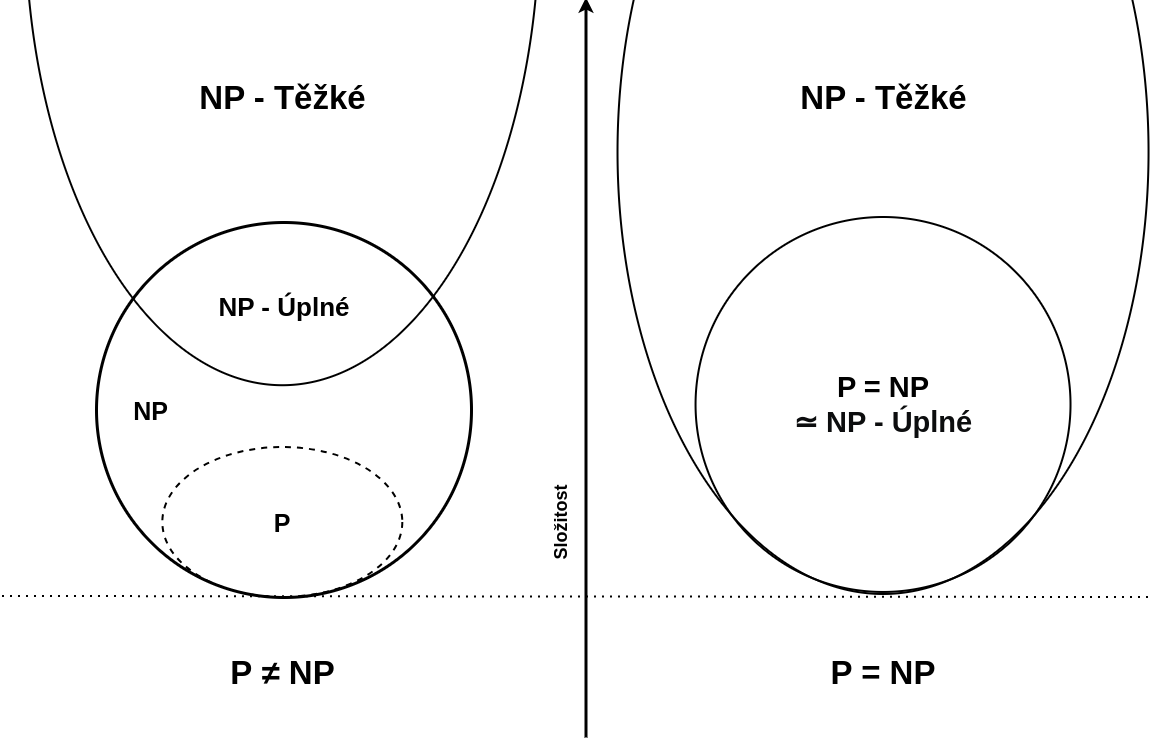
\includegraphics[width = 12cm]{Images/HierarchieProblemTrid.png}
    \caption{Hierarchie tříd složitosti}
    \label{fig:HierarchieProblemTrid}
\end{figure}

\section{Neúplné řešení}
Jak bylo řečeno dříve, hledání Hamiltonovské kružnice patří mezi \(NP\)- úplné problémy, tedy že pro obecný graf neumíme najít Hamiltonovskou kružnici efektivně. Jsme schopni nalézt takovou kružnici v časové složitosti \(O(n!)\), to znamená, že pro velmi malá \(n\) dokáže-\\me najít kružnici celkem rychle, ale třeba už pro \(n = 17\) by výpočet trval přibližně 4 dny. 

Graf používaný ve hře Snake je čtvercový. Omezení daná z jeho definice nám usnadní úlohu hledání kružnice, protože problém již nemusíme řešit pro obecný graf, který má mnohem více hran. Pro čtvercový graf jde relativně snadno najít Hamiltonovská kružnice, pomocí algoritmu od Johna Tapsella~\cite{tapsell2025snake}.

\subsection{Algoritmus poloviční kostry grafu}

Nejdůležitější myšlenka algoritmu pro hledání Hamiltonovské kružnice ve čtvercovém grafu se zakládá na kostře grafu (Obrázek~\ref{fig:SpanningTreeSmallerGraph}). Pokud se pozorně podíváme na kostru nějakého čtvercového grafu, zjistíme, že obvod kostry je vlastně Hamiltonovská kružnice pro graf dvakrát větší (Obrázek~\ref{fig:SpanningTreeToHamilton}). To znamená, že pro nalezení kružnice potřebujeme vygenerovat kostru pro graf s dvakrát menšími rozměry než má graf, ve kterém se snažíme najít kružnici. 

\begin{figure}[!ht]
    \centering
    \begin{subfigure}[t]{0.45\textwidth}
        \centering
        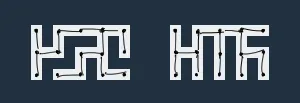
\includegraphics[width=\textwidth]{Images/SpanningTreeSmallerGraph.png}
        \caption{Kostry grafu}
        \label{fig:SpanningTreeSmallerGraph}
    \end{subfigure}
    \hfill
    \begin{subfigure}[t]{0.45\textwidth}
        \centering
        
\includegraphics[width=\textwidth]{Images/SpanningTreeToHamilton.png}
        \caption{Transformace z kostry na Hamiltonovskou kružnici}
        \label{fig:SpanningTreeToHamilton}
    \end{subfigure}
    \caption[Dostupné z: \url{https://miro.medium.com/v2/resize:fit:600/format:webp/1*kviW8mFsjXoLeOTdqTmbmA.png} \textbf{,}  \url{https://miro.medium.com/v2/resize:fit:600/format:webp/1*aB8mFapIsycDGVueoSpr1Q.png}]{Kostry grafu a jejich transformace}
\end{figure}

Nalezení kostry velmi ulehčuje hledání Hamiltonovské kružnice ve čtvercovém grafu, ale bohužel můžeme tímto způsobem vygenerovat pouze podmnožinu všech možných Hamiltonovských kružnic (Obrázek~\ref{fig:NotAllGenerations}). Zvětšováním rozměrů grafu \(n \times m\), ve kterém hledáme kostru, se zároveň omezuje i velikost grafu, ve kterém následně hledáme Hamilto-\\novskou kružnici – ta je určena rozměry \(2n \times 2m\).

Pro úspěšné vyřešení hry Snake ovšem nepotřebujeme najít všechny možné Hamiltonovské kružnice, stačí nám alespoň jedna. Proto můžeme přístup založený na hledání kostry grafu bez obav využít.

\begin{figure}[!t]
    \centering
    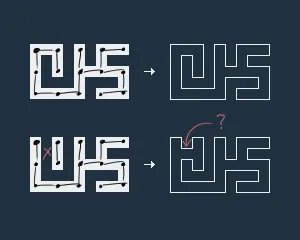
\includegraphics[width = 0.8\textwidth]{Images/NotAllGenerations.png}
    \caption[Dostupné z: \url{https://miro.medium.com/v2/resize:fit:600/format:webp/1*P8932ZvcHs8vOl3OXzJCnA.png}]{Kostra grafu, která neumožňuje vygenerovat všechny možné Hamiltonovské kružnice, ale pouze jejich podmnožinu}
    \label{fig:NotAllGenerations}
\end{figure}

\subsection{Nález Hamiltonovské kružnice}

Díky algoritmu popsanému v předchozí sekci dokážeme snadno najít Hamiltonovskou kružnici, jako obvod kostry dvakrát menšího grafu. Jak ale v praxi vytvoříme graf jako obvod kostry? 

První, co si musíme uvědomit, je, že každý vrchol z menšího grafu má okolo sebe vždy čtyři vrcholy většího grafu. Ke každému vrcholu musíme tedy správně přiřadit čtyři vrcholy většího grafu. Zkusme přemýšlet nad konkrétním příkladem.

Graf, ve kterém budeme hledat kostru, bude mít rozměry \(3 \times 3\), tím pádem graf, ve kterém se budeme snažit najít kružnici, má rozměry \(6 \times 6\). Vrcholy budeme číslovat od nuly, menší graf bude mít vrcholy 0-8, větší graf 0-35. Z Obrázku~\ref{fig:HledaniKruzniceZKostry} je patrné, že stačí zjistit číslo vrcholu, který je od vrcholu menšího grafu umístěn vlevo nahoře, protože ostatní tři vrcholy dokážeme zjistit přičtením fixních konstant. Jak se konkrétně přiřadí sousední vrcholy, ilustrujeme pomocí metody \texttt{neighbor\_nodes}~\ref{lst:neighbor_nodes}. 

Když už máme přiřazené sousední vrcholy, stačí zjistit, které z nich potřebujeme spojit, abychom získali Hamiltonovskou kružnici. Z Obrázku~\ref{fig:HledaniKruzniceZKostry} vidíme, že rozhodně můžeme vždy spojit vrcholy, které se nacházejí v rohu hracího pole (v našem případě $[6, 0]$ a $[0, 1]$, nebo $[24, 30]$ a $[30, 31]$ atd.). Další hrany, o kterých určitě víme, že je můžeme vytvořit, jsou hrany mezi vrcholy, které se nacházejí na krajích hracího pole a zároveň sousedí s vrcholy přiřazenými ke stejnému vrcholu z menšího grafu. To jsou např.: $[12, 18]$, $[2, 3]$ nebo $[17, 23]$.

\begin{figure}[H]
    \centering
    \begin{lstlisting}[language=python, style=python, caption={Určení sousedních vrcholů většího grafu}, label={lst:neighbor_nodes}, mathescape=true]
    def neighbor_nodes(self):
        nodes_for_smaller_nodes = {}
        for x in range(self.vertices):
            left_up = ((x // self.number_of_nodes_on_side) 
            * 4 * self.number_of_nodes_on_side)
            + ((x % self.number_of_nodes_on_side) * 2)
            right_up = left_up + 1
            left_down = left_up + (self.number_of_nodes_on_side * 2)
            right_down = left_down + 1
            # Save neighbor nodes into the dictionary
            nodes_for_smaller_nodes[x] = {
                "left_up": left_up,
                "right_up": right_up,
                "left_down": left_down,
                "right_down": right_down
            }
        return nodes_for_smaller_nodes
    \end{lstlisting}
\end{figure}

O ostatních hranách již nemůžeme rozhodnout tak jednoduše bez využití kostry menšího grafu. Vezměme tedy např. hranu z menšího grafu $[0, 1]$, vidíme, že pokud chceme utvořit obrys této hrany, potřebujeme spojit vrcholy nad hranou $[1, 2]$ a pod hranou $[7, 8]$. Tyto hrany jsou rovnoběžné k hraně $[0, 1]$ malého grafu. Kdyby hrana $[0, 1]$ mezi vrcholy malého grafu nebyla, museli bychom spojit sousední vrcholy bodů 0 a 1 ve směru kolmém na hypotetickou hranu $[0, 1]$. To znamená hrany $[1, 7]$ a $[2, 8]$. Takovým způsobem pokračujeme ve stavbě celého grafu. Procházíme všechny vrcholy malého grafu, které tvoří kostru. Pokud existuje hrana mezi dvěma vrcholy v menším grafu, spojíme odpovídající sousední vrcholy v rozšířeném grafu rovnoběžně se směrem této hrany. Pokud v menším grafu hrana neexistuje, spojíme odpovídající sousední vrcholy ve větším grafu ve směru kolmém na směr, ve kterém by tato hrana vedla.

\begin{figure}[H]
    \centering
    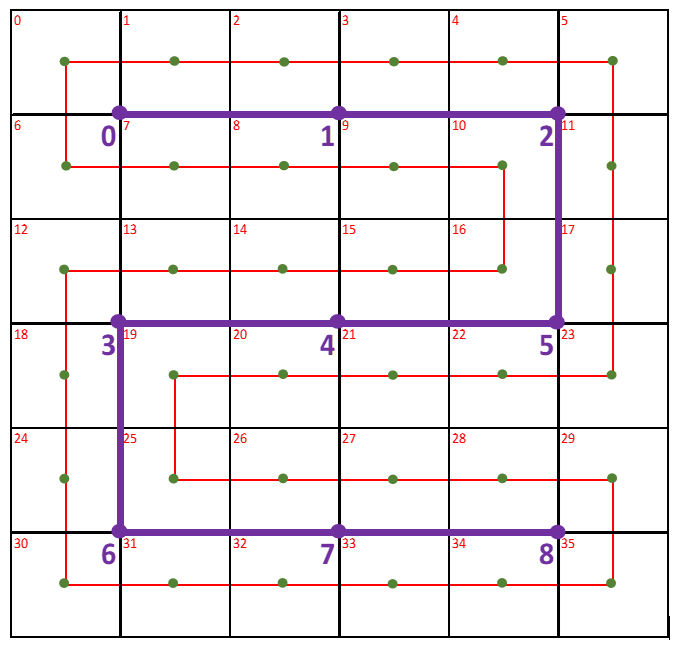
\includegraphics[width=0.7\linewidth]{Images/HledaniKruzniceZKostry.png}
    \caption{Kostra malého grafu, Hamiltonovská kružnice velkého grafu, sousední vrcholy (zelené)}
    \label{fig:HledaniKruzniceZKostry}
\end{figure}

\section{Rychlost řešení hry}

Použití Hamiltonovské kružnice pro úspěšné dokončení hry Snake funguje vždy~\cite{Graafsma2025Snake}. V porovnání s jinými metodami, které budou popsány dále v textu, je ovšem nesmírně pomalé (porovnání v kapitole~\ref{Srovnání algoritmů}). Cílem této práce nebylo pouze úspěšné dokončení hry, ale její dokončení v co nejkratším čase.

Při tomto přístupu k řešení hry se například vůbec neuvažuje nad tím, kde se objeví další jablko. To znamená, že na začátku hry, kdy je had ještě velmi malý, je průměrná vzdálenost, kterou had musí urazit k jablku, polovina hracího pole, neboli  \(\frac{n}{2}\) všech vrcholů v grafu. V polovině hry, kdy had zabírá nějaký prostor, se už jablko musí objevit blíže k hadovi a na konci hry, když had zabírá skoro celé hrací pole, se bude jablko objevovat přímo před ním. K poslednímu jablku, které had sebere, urazí cestu dlouhou jedno políčko.

Tím pádem dokážeme vypočítat průměrný počet tahů na hru při použití Hamiltonovské kružnice pro dokončení hry. Počet tahů vyjádříme následujícím vztahem: 
\begin{center}
    $\frac{\frac{n}{2} \cdot n}{2}$
\end{center}
kde \(n\) je počet vrcholů v grafu (počet políček v herním poli)~\cite{alphaphoenix2020snake}.  Na závislost můžeme nahlédnout také na Obrázku~\ref{fig:HamiltonianCycleDuration}.

\begin{figure}
    \centering
    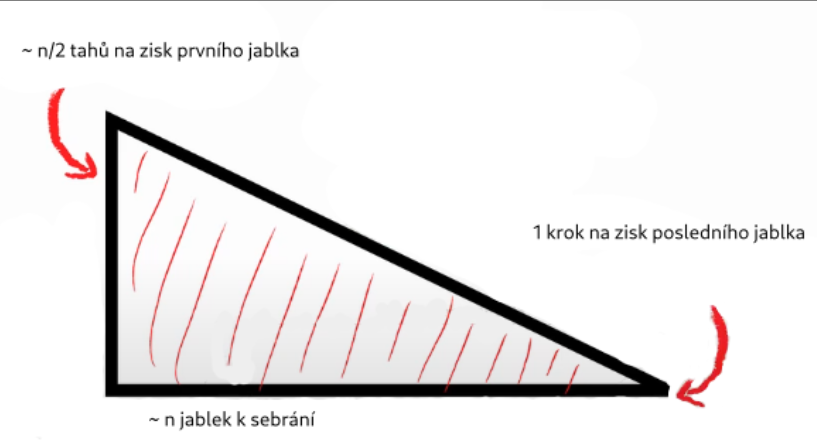
\includegraphics[width=0.7\linewidth]{Images/HamiltonianCycleDuration.png}
    \caption[Dostupné z: \url{https://www.youtube.com/watch?v=TOpBcfbAgPg&t=245s&ab_channel=AlphaPhoenix}]{Výpočet přibližného počtu tahů}
    \label{fig:HamiltonianCycleDuration}
\end{figure}